\subsection{Growth Rates and Dominance Relations}

\begin{figure}[H]
  \centering
     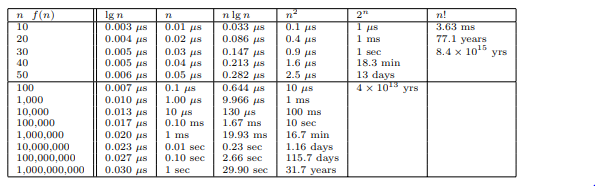
\includegraphics[scale=1.0]{./2_4.png}
  \label{fig:demo-diagram2-4}
  \caption{ Growth rates of common functions measured in nanoseconds}
\end{figure}


\subsubsection{Dominance Relations}

\noindent\fbox{\parbox{\textwidth}{%
\emph{Take-Home Lesson: }Although esoteric functions arise in advanced algorithm
analysis, a small variety of time complexities suffice and account for most
algorithms that are widely used in practice.
}%
}


